%input macros (i.e. write your own macros file called MacroFile1.tex)
%\include{Macros/MacroFile1}

\documentclass[oneside,12pt]{Classes/CUEDthesisPSnPDF}

\ifpdf
%    \pdfinfo { /Title  (LIT Masters Thesis)
%               /Creator (TeX)
%               /Producer (pdfTeX)
%               /Author (Paul Vesey paul.vesey@lit.ie)
%               /CreationDate (D:20120601000000)  %format D:YYYYMMDDhhmmss
%               /ModDate (D:20120615213532)
%               /Subject (LIT Masters Thesis)
%               /Keywords (PhD, Thesis)}
    \pdfcatalog { /PageMode (/UseOutlines)
                  /OpenAction (fitbh)  }
\fi

\title{LIT Masters Thesis Title}
\stitle{Subtitle of Thesis}
\supervisor{Supervisor}
\formalsupervisor{Dr. Super Visor}
\cosupervisor{Co-Supervisor}
\formalcosupervisor{Dr. Co Supervisor}
\formalauthor{Ms. Anne E. Mal}

\ifpdf
  \author{\href{mailto:paul.vesey@lit.ie}{Paul Vesey}}
  \collegeordept{\href{http://www.lit.ie/BuiEnv/}{School of the Built Environment}}
  \university{\href{http://www.lit.ie}{Limerick Institute of Technology}}
% insert below the file name that contains the crest in-place of 'UnivShield'
  \crest{\includegraphics[width=90mm]{SBE.jpg}}

\else
  \author{Paul Vesey}
  \collegeordept{School of the Built Environment}
  \university{Limerick Institute of Technology}
% insert below the file name that contains the crest in-place of 'UnivShield'
  \crest{\includegraphics[bb = 0 0 292 336, width=90mm]{SBE.jpg}}

\fi



%
% insert below the file name that contains the crest in-place of 'UnivShield'
% \crest{\IncludeGraphicsW{UnivShield}{40mm}{14 14 73 81}}
%
%\renewcommand{\submittedtext}{change the default text here if needed}
\degree{Master of Science}
\degreedate{Yet to be decided}

% turn of those nasty overfull and underfull hboxes
\hbadness=10000
\hfuzz=50pt

% Put all the style files you want in the directory StyleFiles and usepackage like this:
%\usepackage{StyleFiles/watermark}
%\usepackage{watermark}


% Comment out the next line to get single spacing
\onehalfspacing

\begin{document}

%\language{english}

% A page with the abstract on including title and author etc may be
% required to be handed in separately. If this is not so, then comment
% the below 3 lines (between '\begin{abstractseparte}' and 
% 'end{abstractseparate}'), normally like a declaration ... needs some more
% work, mind as environment abstracts creates a new page!
% \begin{abstractseparate}
%   \input{Abstract/abstract}
% \end{abstractseparate}




% Using the watermark package which is in StyleFiles/
% and to remove DRAFT COPY ONLY appearing on the top of all pages comment out below line
%\watermark{DRAFT COPY ONLY}


\maketitle

%set the number of sectioning levels that get number and appear in the contents
\setcounter{secnumdepth}{3}
\setcounter{tocdepth}{3}

\frontmatter % book mode only
\pagenumbering{roman}
% Thesis Declaration ---------------------------------------------------

\begin{declaration} %this creates the heading for the dedication page


The work presented in this thesis is the original work of the author, under the direction of \@formalsupervisor and due reference has been made, where necessary, to the work of others. No part of this thesis has been previously submitted to LIT or any other Institute.

\vspace{3cm}

\begin{flushleft}
\makebox[4.5cm]{\hrulefill}  \hfill Date: \makebox[2.5cm]{\hrulefill}\\


\textit{\@formalauthor}, \\
Research Candidate \\ 
\end{flushleft}



\vspace{2cm}

\begin{flushleft}
\makebox[4.5cm]{\hrulefill}  \hfill Date: \emph{\today} \\
\textit{\@formalsupervisor},\\
Lead Supervisor \\ 
\end{flushleft}


\end{declaration}

% ----------------------------------------------------------------------

%%% Local Variables: 
%%% mode: latex
%%% TeX-master: "../thesis"
%%% End: 

\include{Dedication/dedication}
\include{Acknowledgement/acknowledgement}
\include{Abstract/abstract}

\tableofcontents
\listoffigures
\printnomenclature  %% Print the nomenclature
\addcontentsline{toc}{chapter}{Nomenclature}

\mainmatter % book mode only
\include{Introduction/introduction}
% \pagebreak[4]
% \hspace*{1cm}
% \pagebreak[4]
% \hspace*{1cm}
% \pagebreak[4]

\chapter{My First Chapter But Note The Numbering ...}
\ifpdf
    \graphicspath{{Chapter1/Chapter1Figs/PNG/}{Chapter1/Chapter1Figs/PDF/}{Chapter1/Chapter1Figs/}}
\else
    \graphicspath{{Chapter1/Chapter1Figs/EPS/}{Chapter1/Chapter1Figs/}}
\fi
\markboth{\MakeUppercase{\thechapter. My First Chapter }}{\thechapter. My First Chapter}

\section{First Paragraph}

And now I begin my first chapter here ...

Here is an equation\footnote{the notation is explained in the nomenclature section :-)}:
\begin{eqnarray}
CIF: \hspace*{5mm}F_0^j(a) &=& \frac{1}{2\pi \iota} \oint_{\gamma} \frac{F_0^j(z)}{z - a} dz
\end{eqnarray}
\nomenclature[zcif]{$CIF$}{Cauchy's Integral Formula}                                % first letter Z is for Acronyms 
\nomenclature[aF]{$F$}{complex function}                                                   % first letter A is for Roman symbols
\nomenclature[gp]{$\pi$}{ $\simeq 3.14\ldots$}                                             % first letter G is for Greek Symbols
\nomenclature[gi]{$\iota$}{unit imaginary number $\sqrt{-1}$}                      % first letter G is for Greek Symbols
\nomenclature[gg]{$\gamma$}{a simply closed curve on a complex plane}  % first letter G is for Greek Symbols
\nomenclature[xi]{$\oint_\gamma$}{integration around a curve $\gamma$} % first letter X is for Other Symbols
\nomenclature[rj]{$j$}{superscript index}                                                       % first letter R is for superscripts
\nomenclature[s0]{$0$}{subscript index}                                                        % first letter S is for subscripts

\section{Second Paragraph}
and here I write more ...\cite{texbook}

\subsection{Mendeley}

Mendeley is not necessary for \LaTeX.  Mendeley is a standalone referencing management system that can be integrated to Microsoft Word or with \LaTeX.  The Mendeley application will manage your references in a manner similar to EndNote.  The major advantage of Mendeley is that it will also manage your downloaded .pdf files.  For more details of Mendeley and its functionality please go to \href{http://www.mendeley.com/}{www.mendeley.com} 





\subsection{MiKTeX}

The MiKTeX distribution contains the source files and executables for \LaTeX  to work.  The MiKTex distribution comes is available  from \href{http://miktex.org/}{miktex.org}  Please note that a completed installation will consume approx 2.0 Gig of hard disk space.  As the system is based on 'packages' you can elect to download and install packages as they are required.  This will substantially reduce the hard disk requirement; however it can pose problems when internet connectivity is lost.  My preferred option is to install the full distribution.  


\subsection{TeXnicCenter}

In order to use \LaTeX you will need a text editor.  There are numerous editors available for free download.  To date I have found TeXnicCenter to be the most flexible.  TeXnicCenter is available from  \href{http://www.texniccenter.org/}{www.texniccenter.org} 






\subsection{Referencing and Citation}
... and some more ...

Now I would like to cite the following: \cite{latex} and \cite{texbook}
and \cite{Rud73}.

Referencing or citation can be achieved in a number of formats.  The standard is the \verb|\cite| command which will display as above.  Alternatives are \verb|\citet| and   \verb|\citep|.  The \verb|\citet| command produces \citet{KR83} whereas the \verb|\citep| command produces \citep{latex}.  More information is available from the  \href{http://merkel.zoneo.net/Latex/natbib.php}{Natbib Reference Sheet by Ross Moore}

\subsection{Including Figures and Pictures}


I would also like to include a picture ...

\begin{figure}[!htbp]
  \begin{center}
    \leavevmode
    \ifpdf
      \includegraphics[height=6in]{aflow}
    \else
      \includegraphics[bb = 92 86 545 742, height=6in]{aflow}
    \fi
    \caption{Airfoil Picture}
    \label{FigAir}
  \end{center}
\end{figure}

% above code has been macro-fied in Classes/MacroFile.tex file
%\InsertFig{\IncludeGraphicsH{aflow}{6in}{92 86 545 742}}{Airfoil Picture}{FigAir}

So as we have now labelled it we can reference it, like so (\ref{FigAir}) and it
is on Page \pageref{FigAir}. And as we can see, it is a very nice picture and we
can talk about it all we want and when we are tired we can move on to the next
chapter ...

I would also like to add an extra bookmark in acroread like so ...
\ifpdf
  \pdfbookmark[2]{bookmark text is here}{And this is what I want bookmarked}
\fi
% ------------------------------------------------------------------------


%%% Local Variables: 
%%% mode: latex
%%% TeX-master: "../thesis"
%%% End: 

\chapter{My Second Chapter}
\ifpdf
    \graphicspath{{Chapter2/Chapter2Figs/PNG/}{Chapter2/Chapter2Figs/PDF/}{Chapter2/Chapter2Figs/}}
\else
    \graphicspath{{Chapter2/Chapter2Figs/EPS/}{Chapter2/Chapter2Figs/}}
\fi

\markboth{\MakeUppercase{\thechapter. My Second Chapter }}{\thechapter. My Second Chapter}


\section{Some Standard things that you may need}

\subsection{Tables}

This subsection contains a few examples of tables such as table \ref{tab:TestTable} and table \ref{tab:StatusData}.  It also shows a use case for the tabularx environment shown in table \ref{tab:tabularx}.\\


\begin{table}[ht]
	\centering
	\begin{tabular}{|c|c|}
		\hline
		Item & Entry \\
		\hline
		Item  & Entry \\
		\hline
	\end{tabular}
	\caption{Table Name}
	\label{tab:TestTable}
\end{table}

\begin{table}[ht]
	\begin{tabularx}{\textwidth}{ |X|X| }
		\hline
		\textbf{Important stuff:} & As stated \\
		\hline 
		\textbf{More Important Stuff:}  & As stated  \\
		\hline
	
	\end{tabularx}
	\caption{tab:Using TabularX}
	\label{tab:tabularx}
\end{table}

\begin{table}[ht]
	\centering
	\begin{tabular}{ |c|r| }
		\hline
		\textbf{No.} & \textbf{Status Data} \\
		\hline 
		1 &  Some \\ 
		2 &  Data \\ 
		3 &  shown\\ 
		4 &  here \\
		\hline
	\end{tabular}
	\caption{Status Data}	
	\label{tab:StatusData}
\end{table}


\subsection{Figures}

Generally, images are pretty simple.  Use .jpg or png and you will be fine.  Just remember the captions.  If you need to rotate an image, you will have to do slightly more work.  All images here are licences under Creative Commons.

% TODO: \usepackage{graphicx} required
\begin{figure}[ht]
	\centering
	\includegraphics[width=0.7\linewidth]{./jpg/ColorfullSky.jpg}
	\caption[Colorfull Sky]{Colorful clouds and blue sky with water reflection of an island hosting trees at sunrise in Si Phan Don, Laos. Basile Morin, CC BY-SA 4.0}
	\label{fig:ColorSky}
\end{figure}


\begin{sidewaysfigure}[ht]
	\centering
	\includegraphics[width=1.0\linewidth]{./jpg/ColorfullSky.jpg}
	\caption{Sideways Image}
	\label{fig:SidewaysImage}
\end{sidewaysfigure}


\subsection{Vector Graphic Images}
Vector graphics can be handled in two ways.  Firstly, you can use eps files generated in another application, or secondly you can create the images on the fly using tikzpicture. A vector image is shown in figure \ref{fig:VennDiagram}.

\begin{figure}[ht]
	\centering
	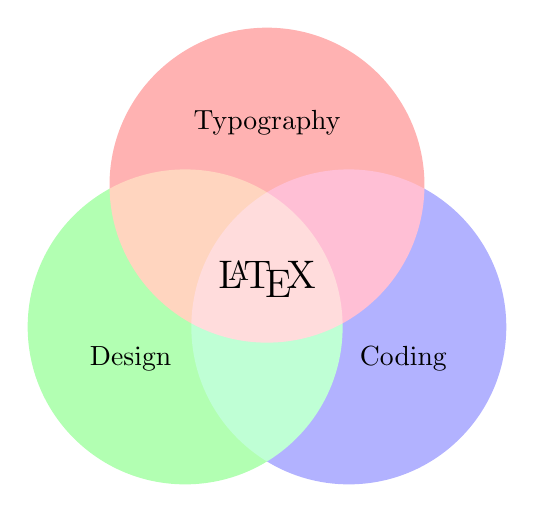
\begin{tikzpicture}
		\begin{scope}[blend group = soft light]
			\fill[red!30!white]   ( 90:1.2) circle (2);
			\fill[green!30!white] (210:1.2) circle (2);
			\fill[blue!30!white]  (330:1.2) circle (2);
		\end{scope}
		\node at ( 90:2)    {Typography};
		\node at ( 210:2)   {Design};
		\node at ( 330:2)   {Coding};
		\node [font=\Large] {\LaTeX};
	\end{tikzpicture}
	\label{fig:VennDiagram}
	\caption{More Vector examples from: \href{https://texample.net/tikz/examples/all/}{https://texample.net/tikz/examples/all/}}
\end{figure}

\newpage
\section{Computer Code}

\subsection{No Code Highlighting}
There are a few useful options for code also.  If you just want a simple listing, without code highlighting, then 'verbatium' is a good option.  You will have to convert tabs to 4 spaces.
\begin{verbatim}
def scope_test():
    def do_local():
        spam = "local spam"
	
    def do_nonlocal():
        nonlocal spam
        spam = "nonlocal spam"
	
    def do_global():
        global spam
        spam = "global spam"
	
    spam = "test spam"
    do_local()
    print("After local assignment:", spam)
    do_nonlocal()
    print("After nonlocal assignment:", spam)
    do_global()
    print("After global assignment:", spam)
	
    scope_test()
    print("In global scope:", spam)
\end{verbatim}


\subsection{Code Highlighting}

The Listings package will add code highlighting for you, but will not add color. The example shown is for Python; this can be changed to other languages by setting the language correctly.


\begin{lstlisting}[language=Python]
	import numpy as np
	
	def incmatrix(genl1,genl2):
	m = len(genl1)
	n = len(genl2)
	M = None #to become the incidence matrix
	VT = np.zeros((n*m,1), int)  #dummy variable
	
	#compute the bitwise xor matrix
	M1 = bitxormatrix(genl1)
	M2 = np.triu(bitxormatrix(genl2),1) 
	
	for i in range(m-1):
	for j in range(i+1, m):
	[r,c] = np.where(M2 == M1[i,j])
	for k in range(len(r)):
	VT[(i)*n + r[k]] = 1;
	VT[(i)*n + c[k]] = 1;
	VT[(j)*n + r[k]] = 1;
	VT[(j)*n + c[k]] = 1;
	
	if M is None:
	M = np.copy(VT)
	else:
	M = np.concatenate((M, VT), 1)
	
	VT = np.zeros((n*m,1), int)
	
	return M
\end{lstlisting}

The lstlisting environment can be customised to show color syntax highlighting, but it takes a bit of work and is specific to the language.  A good tutorial is here \href{https://denbeke.be/blog/programming/syntax-highlighting-in-latex/}{https://denbeke.be/blog/programming/syntax-highlighting-in-latex/}



\include{Chapter3/chapter3}
\include{Conclusions/conclusions}

\backmatter % book mode only

\bibliographystyle{plainnat}
%\bibliographystyle{Classes/CUEDbiblio}
%\bibliographystyle{Classes/jmb}
%\bibliographystyle{Classes/jmb} % bibliography style
\renewcommand{\bibname}{References} % changes default name Bibliography to References
\bibliography{References/references} % References file

\appendix
%\setcounter{page}{1}

\chapter{Appendix A}
\setcounter{page}{1}
\renewcommand{\thepage}{A-\arabic{page}}
\markboth{\MakeUppercase{Appendix A }}{Appendix A}


Lorem ipsum dolor sit amet, consectetur adipiscing elit. Aenean condimentum ultricies rhoncus. Nullam feugiat, enim rhoncus venenatis interdum, libero neque tempor tellus, quis blandit nisi augue ac augue. Etiam congue, arcu eget ultrices convallis, eros odio interdum nunc, vel facilisis est purus a nisl. Suspendisse egestas pharetra sapien, sed lobortis velit accumsan id. Aenean volutpat orci a urna tincidunt id hendrerit leo suscipit. Curabitur vitae tellus justo. Vivamus nec neque in libero molestie lobortis. Donec pharetra nibh in diam tristique vel commodo tellus dictum. In hac habitasse platea dictumst. Donec varius, lacus sed vulputate suscipit, enim velit aliquet quam, nec lacinia ipsum nunc at felis. Phasellus eget cursus neque. Phasellus rhoncus consectetur tincidunt. Morbi diam justo, viverra lobortis tempor eget, pretium at enim. Integer non erat sit amet metus gravida gravida blandit eu lorem. Vestibulum posuere neque in orci iaculis dignissim.

Sed sit amet enim libero. Proin vel leo ut lacus suscipit tincidunt id commodo nulla. Sed bibendum elit a nibh accumsan fermentum. Integer iaculis orci et magna commodo ac pulvinar turpis porttitor. Pellentesque ornare fringilla eros mattis luctus. Donec consequat, erat in consectetur congue, orci ipsum tempus erat, vitae pellentesque urna nibh non sapien. Suspendisse tincidunt magna eu odio hendrerit eget suscipit risus aliquet. Proin lacus libero, vehicula et pulvinar eu, iaculis et leo. Phasellus posuere elit ut ligula luctus a congue dolor tincidunt. Vestibulum pulvinar adipiscing diam vel venenatis. Duis tempor accumsan ante ut feugiat. Nulla commodo, erat vehicula commodo dictum, nisi dui auctor mi, quis ullamcorper augue justo quis ligula. Pellentesque dolor lorem, mattis sed convallis eu, gravida ut magna.

Duis vel nisi libero. Fusce quis dolor lectus, vitae sagittis mi. Phasellus auctor urna ac enim sagittis at malesuada nulla posuere. Nulla quam nulla, mollis et aliquam a, ornare ac libero. Cras ultrices mauris fermentum est commodo ultrices. Morbi facilisis risus vitae arcu pellentesque a mattis eros aliquet. Mauris feugiat euismod urna fringilla commodo. Proin sollicitudin, sem a egestas interdum, nunc dolor facilisis nunc, et porta urna turpis in lorem. Praesent ultricies pharetra justo, eu vulputate lorem porta quis. Aenean et viverra metus. Nulla augue quam, tincidunt at ullamcorper ac, congue sed felis. Proin viverra porttitor magna, vel volutpat libero sagittis vitae. Donec ultricies risus id lorem placerat nec consequat magna tempor. Nulla leo urna, congue nec dictum in, tincidunt eu nisi.

Nulla at massa sapien. Integer mauris arcu, condimentum volutpat rhoncus non, convallis a leo. In hac habitasse platea dictumst. Praesent dignissim rhoncus risus, mollis ornare enim ultrices vitae. Donec sit amet neque in magna lobortis viverra. Fusce convallis hendrerit scelerisque. Cras ac nibh in justo interdum hendrerit. In a orci ac ligula fringilla tristique. Aenean nec magna augue, in tincidunt turpis. Etiam in metus nulla, eget aliquam libero. Donec consectetur massa ut sapien elementum molestie.

Curabitur ut ante augue, in suscipit magna. In vel neque eu erat hendrerit ornare sit amet condimentum nibh. Nulla ut urna tempus risus tristique egestas ultrices sed ante. Pellentesque molestie arcu eget odio adipiscing ac faucibus nisi dignissim. Quisque sit amet ipsum at nulla adipiscing accumsan in pulvinar ipsum. Nulla facilisi. Donec ultrices rhoncus orci vitae feugiat. Curabitur justo odio, vehicula vitae tincidunt et, condimentum ut sapien. Vestibulum vitae magna magna, et pellentesque nisi. Duis semper erat in purus aliquet quis interdum turpis aliquam. Ut tortor nulla, pretium nec ornare sit amet, ullamcorper nec magna.

Nullam in est enim, sed pretium ante. Maecenas a velit erat. Integer tristique volutpat ligula ac tincidunt. Pellentesque sit amet lobortis risus. Nam ullamcorper orci a arcu posuere semper porta turpis adipiscing. Suspendisse eget lobortis dolor. Proin nec ante nibh, vitae congue magna. Sed commodo, lorem eu feugiat imperdiet, sapien risus consequat quam, id eleifend augue dolor et justo. Mauris vehicula, orci at fermentum condimentum, dolor dolor aliquet massa, in porta sapien nulla eu sem. Mauris mollis iaculis nulla, sed laoreet nisl fringilla a. Aenean quis nunc ac urna hendrerit tempor ut et mi. Aliquam fringilla, est ac mattis sodales, magna lectus commodo turpis, eu iaculis dolor felis in felis. Integer cursus fermentum eros quis consequat. Mauris vitae ante quis odio vulputate vulputate ut nec quam. Donec venenatis, mi congue aliquam lobortis, eros leo convallis diam, in vehicula erat metus et est.

Nam libero lacus, suscipit id tincidunt et, sollicitudin id justo. Donec et sapien diam. Fusce faucibus pharetra nibh, vel mattis risus condimentum sed. Donec ut bibendum ipsum. Donec porta varius odio in condimentum. Vivamus vitae quam tortor, et porttitor ligula. Curabitur vehicula fringilla elit nec pretium. Mauris sed enim sit amet lacus bibendum cursus imperdiet ut nibh. Pellentesque sed odio a lorem semper egestas. Integer rutrum nulla sed tortor aliquam ac rhoncus enim condimentum. Proin sagittis suscipit eros eu semper.

Mauris eleifend est non lacus pharetra viverra. Duis vitae risus sit amet tortor placerat euismod. Morbi vel sapien ante. In hac habitasse platea dictumst. Donec volutpat velit a velit malesuada viverra. Fusce non leo dui, vitae tempor justo. Suspendisse potenti. Donec lobortis ornare scelerisque. Nullam commodo ullamcorper libero, ut tincidunt nibh aliquet sed. Class aptent taciti sociosqu ad litora torquent per conubia nostra, per inceptos himenaeos. Morbi nisl quam, malesuada vitae tempor vel, malesuada eget arcu. Curabitur purus turpis, elementum venenatis sollicitudin sed, vestibulum non nisi.

Morbi vitae tortor vel libero tincidunt aliquam. Suspendisse quis nibh at felis consectetur vulputate. Lorem ipsum dolor sit amet, consectetur adipiscing elit. Aenean dapibus luctus cursus. Lorem ipsum dolor sit amet, consectetur adipiscing elit. Nunc id blandit nisl. Sed at leo suscipit odio condimentum tristique. Curabitur lobortis elit a dui sagittis mattis. Etiam mattis ipsum eu ligula ullamcorper blandit. Vestibulum id placerat dui. Fusce fermentum, ipsum ac tempus fermentum, purus est fermentum massa, eget laoreet elit urna et neque. Curabitur aliquam, ipsum ac gravida aliquet, purus metus tempus neque, vel vestibulum mauris tortor eu lorem. Aenean cursus, magna id bibendum tincidunt, metus lacus ultricies lectus, quis imperdiet ipsum mauris a nisi. Maecenas mi justo, dapibus non volutpat in, ultrices non lectus. Morbi eget volutpat enim. Donec aliquet tortor id dolor vestibulum luctus.

Nam porttitor eros id lacus accumsan molestie mollis lorem lacinia. Ut egestas cursus neque, non porttitor libero facilisis eget. Ut odio mauris, tempor a egestas at, scelerisque quis nibh. Aliquam est sapien, pretium dapibus dapibus nec, pellentesque sed nulla. Quisque pulvinar, metus eget pretium porttitor, ante diam ultrices diam, tempus placerat est magna et elit. In semper risus ut turpis laoreet et eleifend diam hendrerit. Integer vel suscipit urna. Sed sapien lectus, fermentum at sagittis ac, convallis id tellus. Suspendisse eget ligula non purus tristique elementum.

Sed dictum hendrerit mattis. In lectus sem, rhoncus a imperdiet eu, condimentum non nisi. Pellentesque habitant morbi tristique senectus et netus et malesuada fames ac turpis egestas. Mauris eu felis vitae nisl commodo mattis. Duis lectus lorem, blandit vitae mattis vitae, mattis sed ante. Proin vitae mi eget quam placerat viverra eget eget mauris. Nulla facilisi. Aenean sed risus sit amet lectus dictum dictum ut eu quam. Nunc blandit ante ac nulla bibendum consectetur. Maecenas eget augue vitae diam tincidunt dignissim vel et libero. Sed nisi ipsum, auctor eget elementum ultricies, tempor nec justo. Nunc adipiscing dolor vitae nulla vestibulum interdum. Ut tempor turpis sit amet risus commodo cursus. Phasellus dictum imperdiet dignissim.

Fusce hendrerit ante id lectus tempus consequat. In hac habitasse platea dictumst. In posuere turpis ac arcu posuere scelerisque. Class aptent taciti sociosqu ad litora torquent per conubia nostra, per inceptos himenaeos. Duis ultricies, nunc at feugiat posuere, tortor erat viverra erat, nec tempus diam turpis eu urna. Proin massa nibh, eleifend nec varius nec, condimentum eu enim. Pellentesque malesuada nibh vel massa dictum a hendrerit urna tristique. Mauris tortor orci, tempor ut auctor non, accumsan vestibulum leo. Donec dignissim nunc eu lorem porta rutrum. Morbi sem ipsum, semper vel consectetur in, fringilla facilisis nisi. Vestibulum lacus tortor, mollis id adipiscing ut, porttitor eu erat. Phasellus bibendum auctor leo sed blandit. Quisque malesuada lectus eget lorem egestas ut porttitor ligula tincidunt. Nullam vitae diam et nisl accumsan venenatis.

Quisque eros nisl, volutpat sit amet suscipit ultricies, volutpat vitae lorem. Fusce accumsan leo nulla. Duis quis cursus odio. Quisque congue est in odio viverra tempus. Morbi ac neque in nisl rutrum adipiscing et vitae eros. Maecenas ullamcorper ultrices diam et bibendum. Sed accumsan pharetra viverra. Mauris semper nibh id eros viverra feugiat. Pellentesque sed leo ut tellus viverra tincidunt ut dapibus lacus.

Curabitur euismod pellentesque lectus, vel tincidunt tellus tincidunt ac. Suspendisse semper iaculis enim nec rhoncus. Proin sed nulla eros, ac adipiscing arcu. Quisque metus lectus, dapibus eget pulvinar in, aliquet et odio. Quisque ac libero vel ligula malesuada faucibus id id neque. Aenean lobortis fermentum urna, eu rutrum diam laoreet lacinia. Nunc porttitor odio id urna elementum in varius mi rhoncus. Pellentesque volutpat scelerisque porta. Fusce ornare nulla sit amet ligula rhoncus id rhoncus nisi imperdiet. In hac habitasse platea dictumst. Morbi ultrices augue eget lorem varius congue. Suspendisse imperdiet rhoncus est vitae cursus.

Cras rhoncus, massa id dignissim molestie, est lacus tristique augue, nec tincidunt augue erat in sapien. Maecenas enim dui, faucibus ac lobortis in, facilisis elementum lorem. Class aptent taciti sociosqu ad litora torquent per conubia nostra, per inceptos himenaeos. Donec nisl sem, vehicula in ultrices sit amet, cursus a nunc. Quisque suscipit, magna non tincidunt vehicula, neque orci tincidunt tellus, eu dapibus ante enim id tortor. Ut in sapien at quam malesuada scelerisque. Pellentesque ut velit lacus. Integer ac nisl felis. Donec rutrum nisl sed velit fermentum in pulvinar eros tempus. In hac habitasse platea dictumst. Duis leo tellus, placerat et facilisis a, consequat et diam. Nunc molestie adipiscing lobortis. Sed eleifend egestas sapien.

Vestibulum at arcu nec lacus imperdiet malesuada ut in enim. Vestibulum sit amet libero vitae augue molestie tincidunt. Aliquam non commodo mauris. Praesent lacinia commodo erat ut porta. Praesent dapibus leo nec mi aliquet at lacinia ante mattis. Phasellus dui est, suscipit ut porttitor ac, sodales eleifend ante. Morbi at leo eu diam convallis ultrices. Mauris eget turpis libero. Suspendisse quis velit quis nunc imperdiet sagittis. Fusce massa erat, malesuada quis suscipit in, molestie eu odio. Praesent vitae imperdiet justo. Phasellus at lorem diam. Vestibulum ante ipsum primis in faucibus orci luctus et ultrices posuere cubilia Curae; Proin accumsan augue at urna semper vitae auctor nisi interdum. Praesent pulvinar, neque in malesuada sagittis, erat lectus sagittis orci, a congue turpis eros iaculis massa.

Fusce eu erat vel magna posuere lobortis in vel ipsum. Class aptent taciti sociosqu ad litora torquent per conubia nostra, per inceptos himenaeos. Nam id imperdiet nisi. Pellentesque elit justo, suscipit nec congue at, bibendum id turpis. Maecenas ut lacus ipsum, id rutrum purus. Proin suscipit, eros nec dapibus ultricies, nunc elit placerat arcu, vitae laoreet justo odio sed justo. In vitae nisl porta quam molestie tincidunt non vitae urna. Duis blandit suscipit aliquam. Fusce erat turpis, aliquet ut laoreet non, fermentum quis sapien.

Nunc non velit id metus eleifend commodo. Sed ac neque at orci consequat egestas sit amet a felis. Etiam blandit dignissim turpis id egestas. Suspendisse nunc nisi, blandit in pulvinar vitae, bibendum blandit nisl. Vestibulum ante ipsum primis in faucibus orci luctus et ultrices posuere cubilia Curae; Sed quis nisi eros, nec accumsan massa. Fusce placerat euismod mi, nec feugiat dui venenatis ultricies. Ut felis libero, placerat vitae vehicula et, fringilla sit amet ipsum. Curabitur tempus est et tellus vestibulum aliquam. Donec nisl urna, fringilla quis accumsan id, tempus non sapien. Morbi molestie commodo dolor sed pulvinar. Morbi vel tellus condimentum ipsum euismod mattis vel quis eros. Duis augue magna, tincidunt eu imperdiet ut, volutpat in ante.

Nam a iaculis nibh. Duis tempus, sapien ut vehicula fermentum, diam nulla porttitor ligula, id aliquam tortor diam sed nulla. Ut rhoncus, tortor aliquet elementum porttitor, dui magna dignissim urna, nec accumsan metus neque id turpis. Donec velit purus, vestibulum ac consectetur sed, molestie nec eros. Aliquam lectus velit, malesuada eget porta a, commodo ac magna. Etiam luctus, lectus eget commodo suscipit, tortor urna malesuada justo, eu mollis ante augue sed sapien. Nulla et tristique ipsum. Integer sed arcu ante. Nunc vel lorem at risus rutrum feugiat. Praesent orci dui, consectetur eget lobortis eget, adipiscing sed quam. In aliquet odio ut dolor cursus aliquam. Ut molestie molestie cursus. In hac habitasse platea dictumst.

Phasellus ultricies elit quis libero sagittis aliquam. Aliquam at elit non justo feugiat semper pulvinar vitae ligula. Nam ut mi semper nisi pellentesque dictum. Nulla facilisi. In lacus nisi, pellentesque a lobortis in, ornare sit amet metus. Duis aliquam molestie enim nec ullamcorper. Duis porta quam quis mi tempus eu lobortis ante malesuada. Phasellus ullamcorper erat quis velit sollicitudin vestibulum. Duis vestibulum varius magna, eu congue nulla consectetur consectetur. Integer ante libero, mollis sit amet aliquet nec, rutrum rutrum urna. Nulla facilisi. Suspendisse sem est, lobortis non posuere ut, elementum a justo. Pellentesque habitant morbi tristique senectus et netus et malesuada fames ac turpis egestas. Donec pellentesque arcu vitae urna pharetra lacinia.




% ------------------------------------------------------------------------

%%% Local Variables: 
%%% mode: latex
%%% TeX-master: "../thesis"
%%% End: 

\include{Appendix2/appendix2}







\end{document}
